Supporting material is available in the \href{https://drive.google.com/drive/folders/1rxPscm24PQ41dW3EaSxCHFeebt27BfVf}{LAB4 shared folder}.

The purpose of this section is to answer both the checkpoint and report questions of the lab, as well as discuss any relevant results obtained during the experiences.

\subsection{Checkpoint 1: Introduction to LoRa Communication (AT Commands)}

In this first checkpoint, we tested the serial communication between the computer and the RAK module using AT commands.
The module was connected through a USB-to-TTL converter, and we opened the Arduino IDE Serial Monitor at 115200 baud to send the commands and observe the responses.

We first used \texttt{ATZ} to reset the device andobserved its response through the serial connection.
We then executed \texttt{AT+VER=?} to identify the firmware version, \texttt{AT+SN=?} to request the device serial number, and \texttt{ATE} to enable command echo.

As shown in Figure~\ref{fig:chk1-1}, the module reported the firmware version \texttt{RUI\_4.2.1\_RAK3172-E} and confirmed that its current operating mode was LoRa P2P.
Several commands returned \texttt{OK}, indicating successful execution.
We accidentally entered the incomplete command \texttt{AT+VER}, which returned \texttt{AT\_PARAM\_ERROR}.
The parameter error was caused by an incorrectly entered command rather than a failure of the serial connection. The serial-number query returned no value before the following \texttt{OK} response.

These results helped us verify the communication interface and become familiar with the AT commands required to configure the module.

\begin{figure}[htbp]
    \centering
    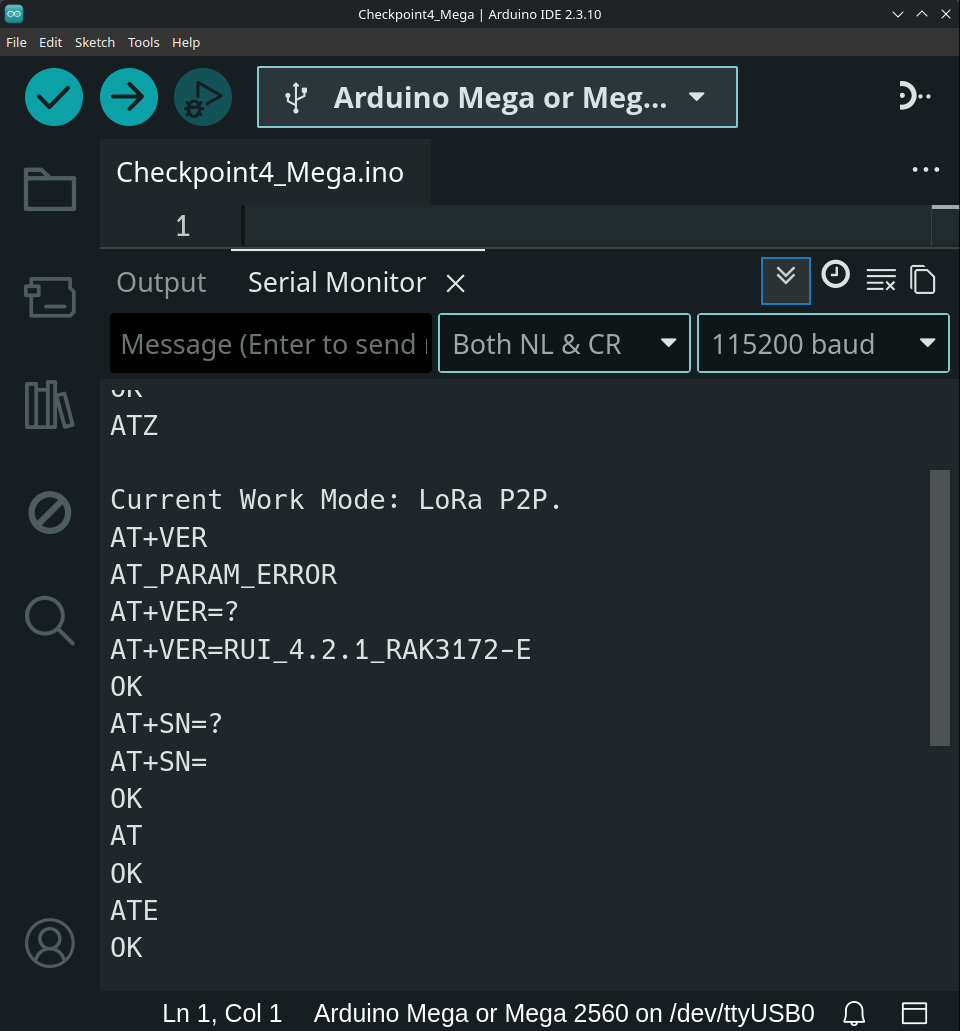
\includegraphics[width=\linewidth]{img/c1.png}
    \caption{Arduino IDE Serial Monitor showing AT command responses, firmware identification, and parameter errors from the RAK module.}
    \label{fig:chk1-1}
\end{figure}

\subsection{Checkpoint 2: Implementation of LoRa P2P Communication}
In this checkpoint, we established a point-to-point communication between two RAK modules, configuring one as the sender and the other as the receiver.
Both modules were connected to their respective computers through USB-to-TTL converters, allowing us to configure and monitor them using AT commands.

First, we used \texttt{AT+NWM=0} to enable LoRa P2P mode on both devices.
We then configured the communication parameters using \texttt{AT+P2P}, making sure that both modules shared the same frequency, spreading factor, bandwidth, coding rate, and preamble length.
The receiver was configured with \texttt{AT+PRECV=65534} to listen continuously, while the sender used \texttt{AT+PRECV=0} before transmitting.
To send a message, we used the command \texttt{AT+PSEND}, followed by the payload encoded in hexadecimal.
The hexadecimal representation is required by the module's AT interface, so the original text must be converted before transmission.

After configuring both RAK modules, we verified their responses through the Arduino IDE Serial Monitor.
Both terminals responded to the AT commands and confirmed that the devices were operating in LoRa P2P mode.
Figure~\ref{fig:chk2-at} shows the recorded output from the sender terminal, including several \texttt{OK} responses and
\texttt{+EVT:TXP2P DONE} events, which indicate completed transmission operations.
Although the same configuration procedure was performed on both devices, only the sender terminal was photographed.
The receiver's output was preserved in a text file and is presented later in this checkpoint.

\begin{figure}[htbp]
    \centering
    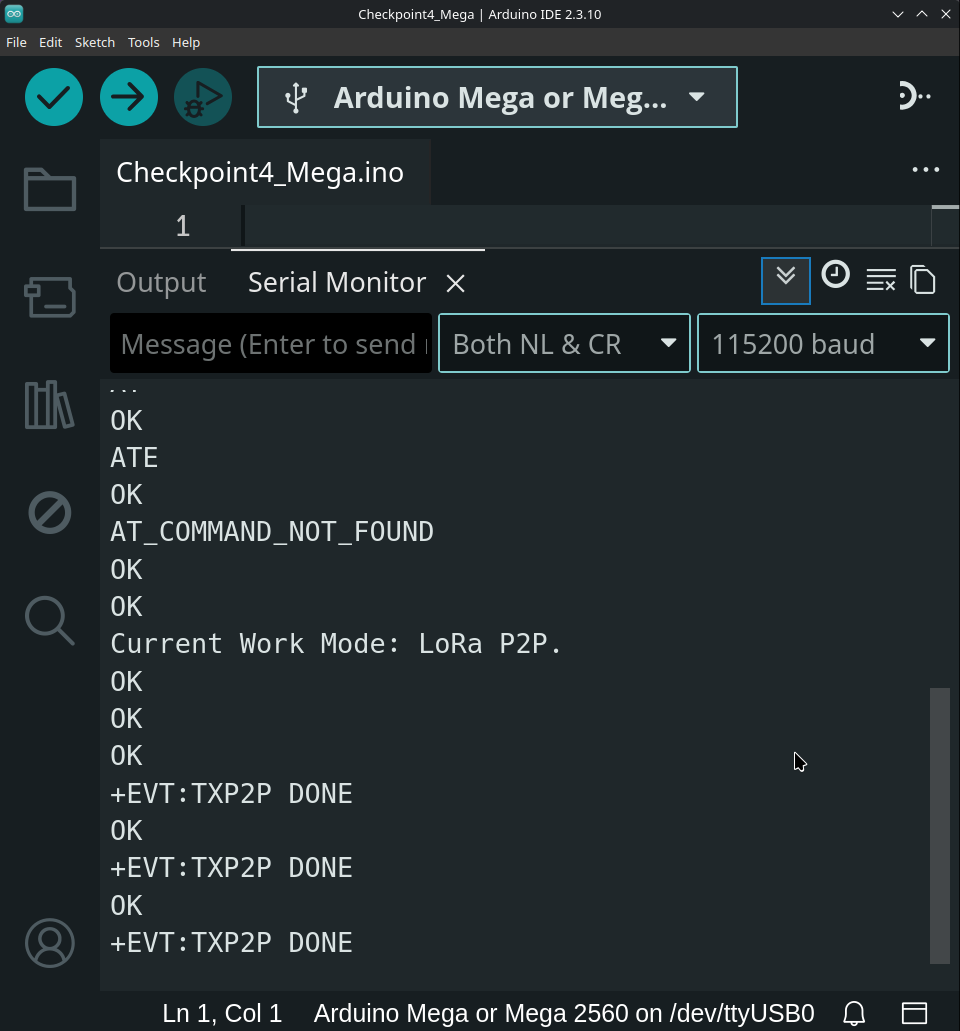
\includegraphics[width=\linewidth]{img/chk2/rak-transmissions.png}
    \caption{RAK module Serial Monitor showing LoRa P2P mode,
    command responses, and completed transmission events.}
    \label{fig:chk2-at}
\end{figure}


Figure~\ref{fig:chk2-1} shows the sender's serial monitor displaying several \texttt{+EVT:TXP2P DONE} events.
These messages indicate that the module completed its transmission operations.
However, they do not independently confirm reception, which must be verified through the receiver's output.

\begin{figure}[htbp]
    \centering
    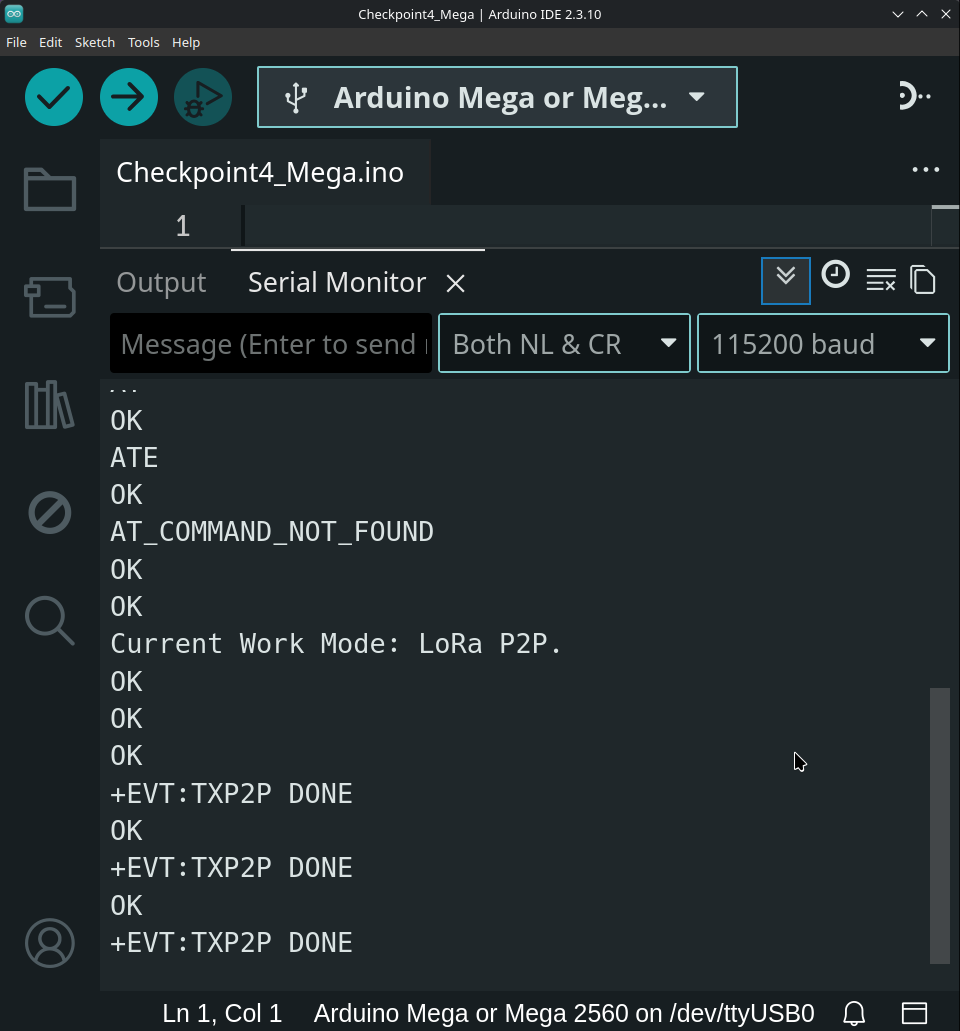
\includegraphics[width=\linewidth]{img/c2.png}
    \caption{Sender Serial Monitor showing successful execution of LoRa P2P transmission operations.}
    \label{fig:chk2-1}
\end{figure}

The physical connection used for the communication test is shown in Figure~\ref{fig:chk2-2}.
The USB-to-TTL converter allowed us to exchange commands and responses with the RAK module through UART, while the antenna was used for wireless transmission.

\begin{figure}[htbp]
    \centering
    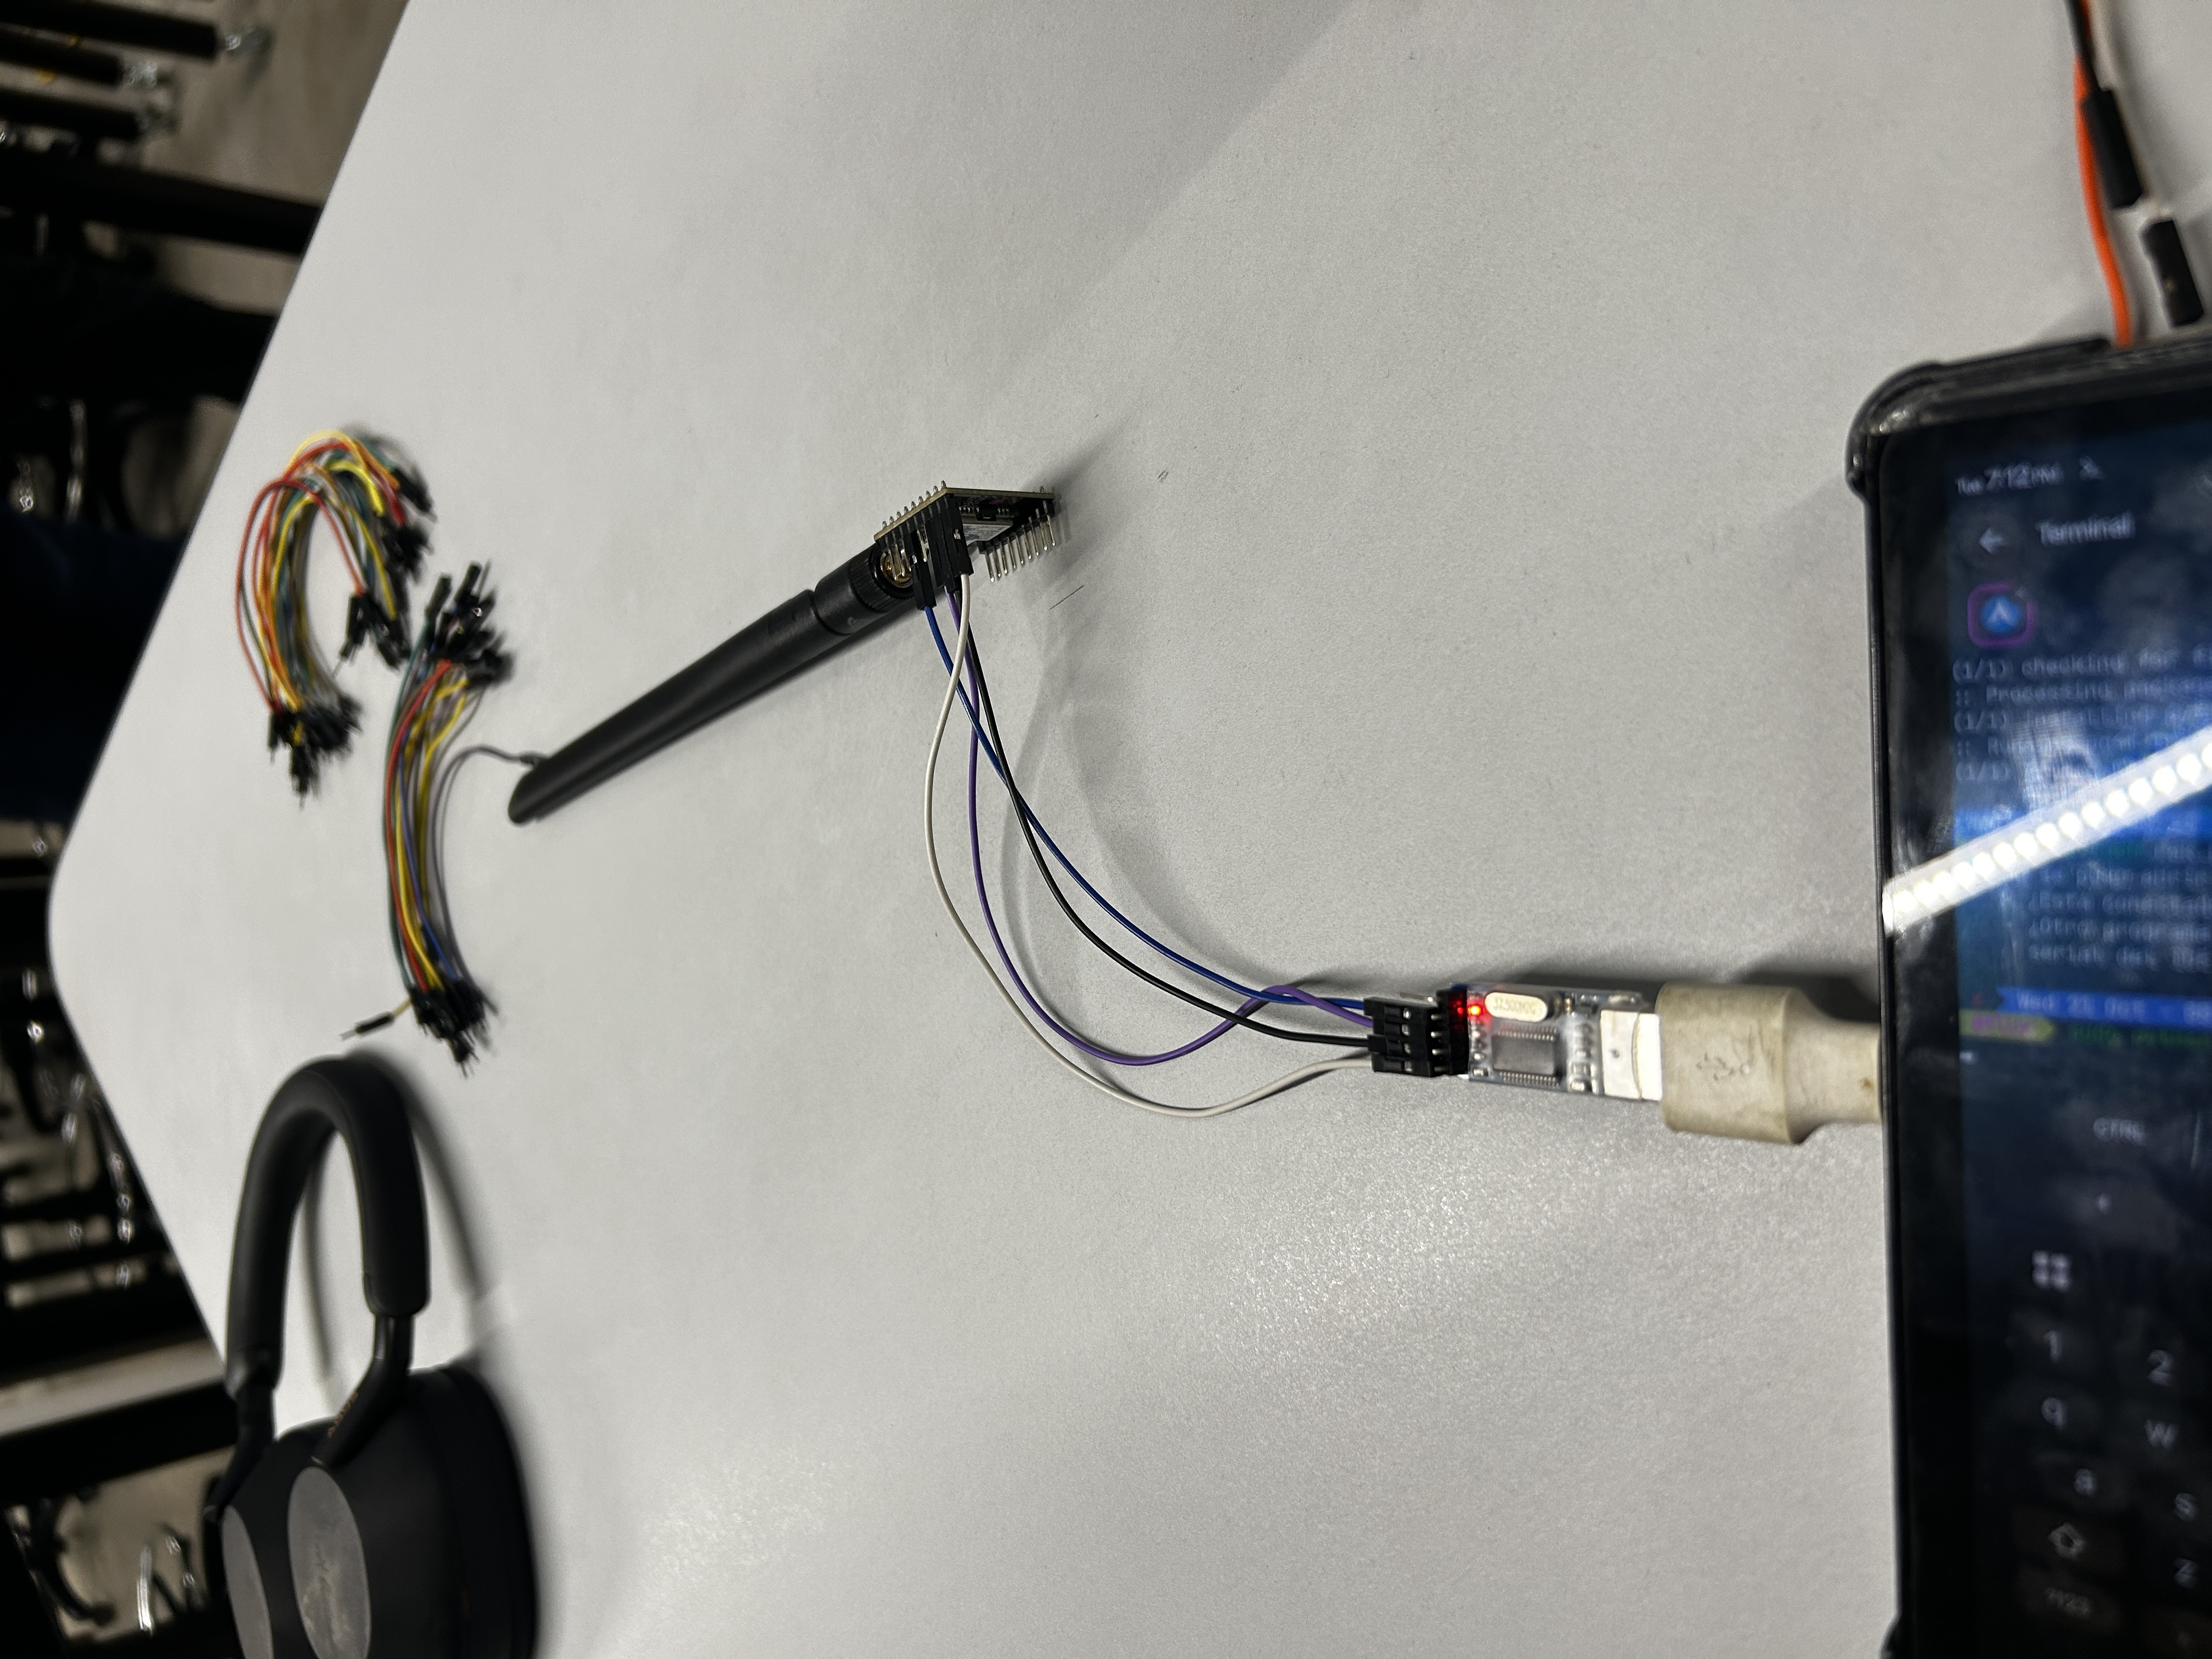
\includegraphics[width=\linewidth]{img/IMG_2477.jpg}
    \caption{RAK module connected through a USB-to-TTL converter for LoRa P2P communication.}
    \label{fig:chk2-2}
\end{figure}

Although we did not capture a photograph of the receiver's serial monitor, we saved its output in a text file.
The recorded results included the following messages:

\begin{lstlisting}[basicstyle=\ttfamily\scriptsize,breaklines=true,columns=fullflexible]
OK
OK
RAKwireless RAK3172-E
\------------------------------------------------------
Version: RUI_4.2.1_RAK3172-E
Current Work Mode: LoRa P2P.
OK
OK
+EVT:RXP2P:-42:8:43
+EVT:RXP2P:-40:8:67
+EVT:RXP2P:-37:8:3637207061706F69
\end{lstlisting}

These messages follow the format \texttt{+EVT:RXP2P:RSSI:SNR:PAYLOAD}, where RSSI represents the received signal strength, SNR indicates the signal-to-noise ratio, and the final field contains the hexadecimal payload.
The recorded RSSI values were -42, -40, and -37 dBm, while the SNR remained at 8 dB for all three messages.
These values confirm that the receiver was detecting the transmissions and reporting their signal characteristics.
Although the RSSI values varied slightly, the available records do not include distance measurements, so this variation cannot be directly attributed to changes in distance.

The first two received messages were test transmissions, while the final message contained the intended text encoded in hexadecimal.
The received payload for the last message was \texttt{3637207061706F69}.
To verify its contents, we converted it from hexadecimal to text, obtaining the message \texttt{67 papoi}, as shown in Figure~\ref{fig:chk2-3}.
This confirms that the received bytes could be decoded into the intended message.

\begin{figure}[htbp]
    \centering
    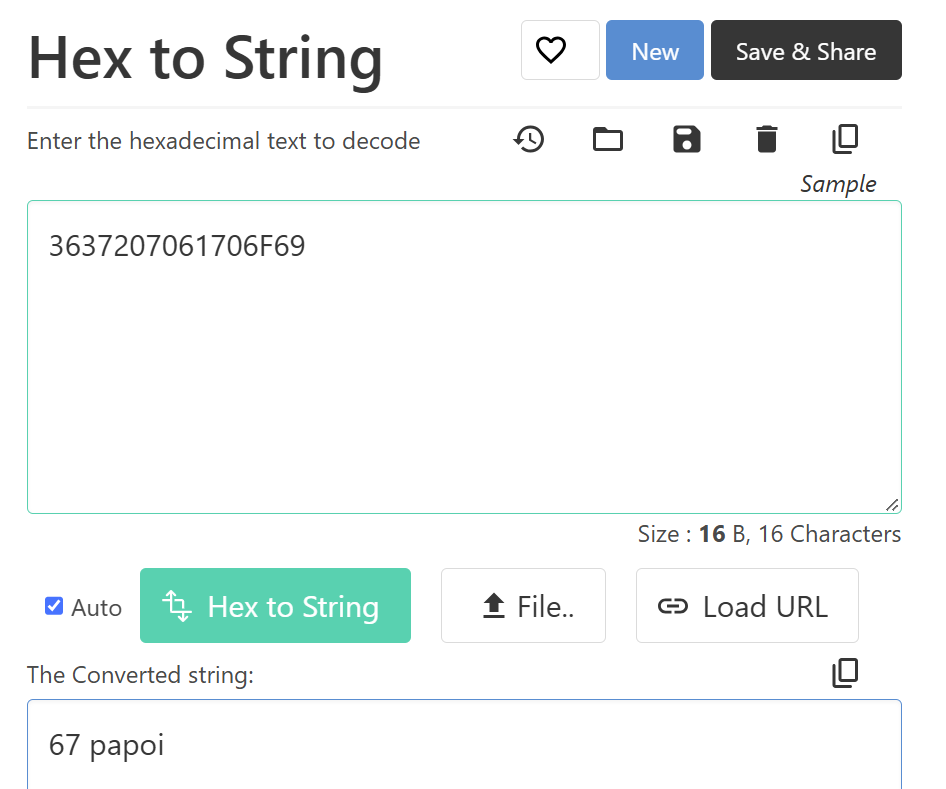
\includegraphics[width=\linewidth]{img/67_papoi.png}
    \caption{Conversion of the received hexadecimal payload into the original text message "67 papoi".}
    \label{fig:chk2-3}
\end{figure}

Overall, the results demonstrate successful communication between the two RAK modules.
The sender reported completed transmissions, while the receiver registered incoming packets containing signal information and hexadecimal payloads.
This allowed us to verify both the wireless communication and the representation of the transmitted data.

The range test was later continued during the automated transmissions in Checkpoint 3. 
The receiver was moved progressively farther from the sender while its received messages and signal measurements were monitored.
Figures~\ref{fig:chk3-receiver} and~\ref{fig:chk3-loss} document the successful receptions and the reception error observed during that demonstration.


\subsubsection{Receiver Measurements}
The record spans 875.078~s, approximately 14.6~minutes. Table~\ref{tab:metrics} summarizes the received samples. The RSSI arithmetic mean is calculated over the reported dBm values and is not an average received power in milliwatts.

\input{\labpath metrics.tex}

Figure~\ref{fig:lora-series} shows the variation of RSSI and SNR over elapsed reception time. Separate panels keep their units distinct. The RSSI ranges from $-116$ to $-22$~dBm, while SNR ranges from $-19$ to $9$~dB. Both values change throughout the record.

\begin{figure}[htbp]
\centering
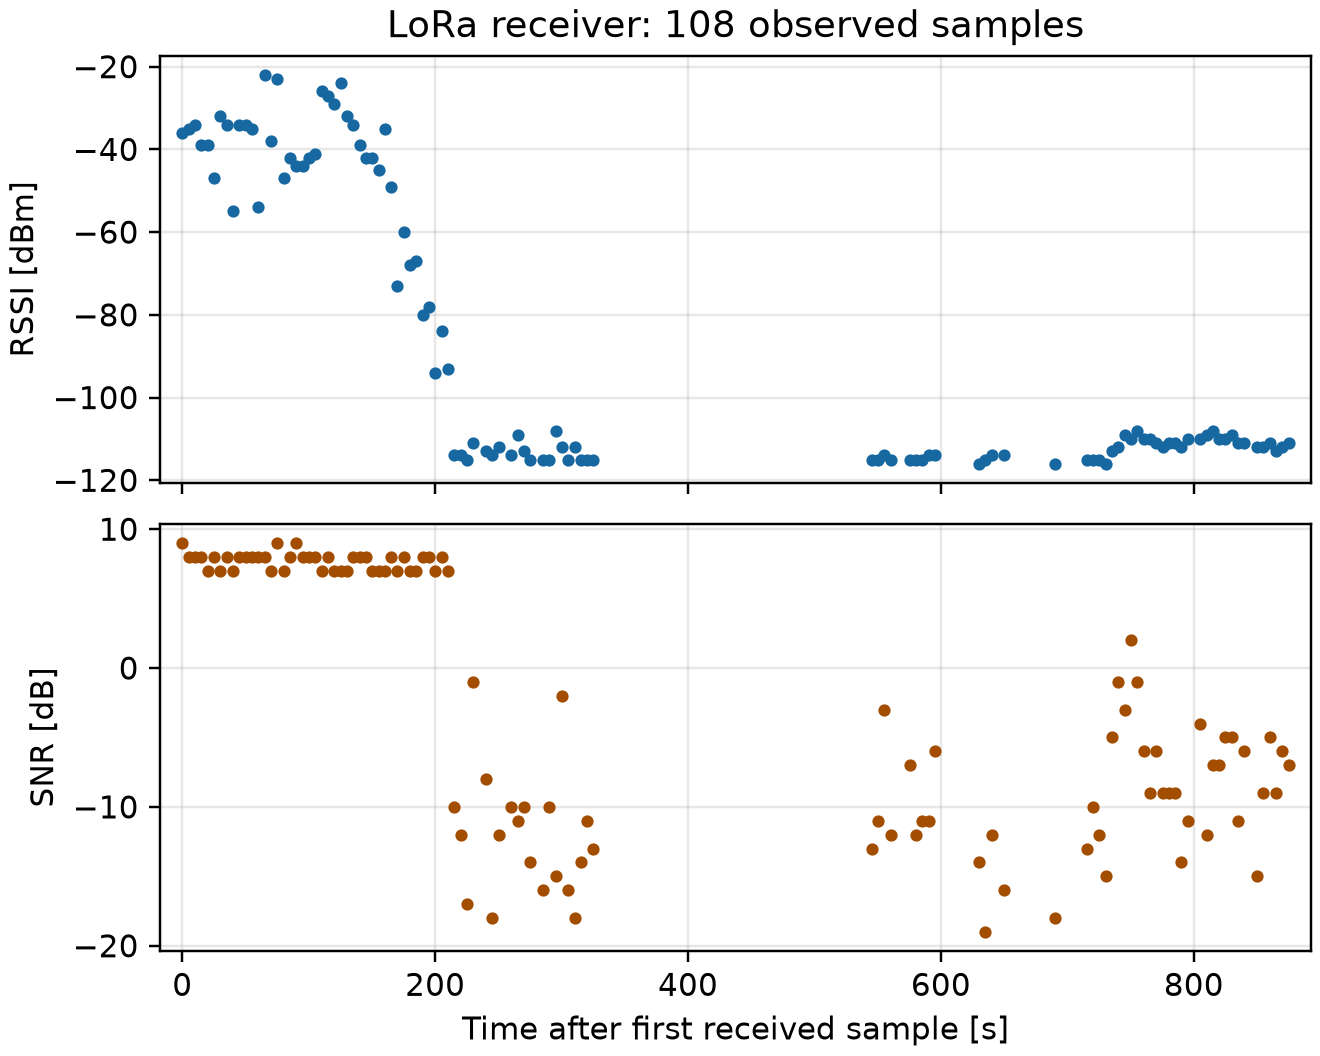
\includegraphics[width=\linewidth]{img/lora-rssi-snr.png}
\caption{RSSI and SNR for 108 received samples, with time relative to the first reception. Markers show individual observations.}
\label{fig:lora-series}
\end{figure}

\Needspace{8\baselineskip}
The low-SNR entries are packets that reached the receiver despite their reported signal-to-noise conditions.
They do not show how many other transmissions were missed.
Empty intervals in the graph contain no recorded observations and cannot, by themselves, establish packet loss.

During the range test, the receiver was progressively moved away from the transmitter while incoming messages were monitored. 
Figure~\ref{fig:lora-series} shows considerable variations in RSSI and SNR throughout the recorded interval,
which are consistent with changes in the radio propagation conditions during the experiment.

However, these variations cannot be attributed exclusively to distance, since obstacles, antenna orientation, and
interference may also affect the received signal.
Furthermore, the receiver's position was not recorded for each sample, so the graph cannot establish an exact relationship between
distance and signal strength or determine the maximum communication range.


\FloatBarrier
\subsection{Checkpoint 3: Integration and Data Transmission with Arduino MEGA}
In this checkpoint, we integrated a RAK LoRa module with an Arduino MEGA to automate the transmission of messages through LoRa P2P communication.
The Arduino was programmed to configure the RAK module and periodically send messages without requiring manual intervention.

\subsubsection{Physical Implementation}
The circuit was assembled using an Arduino MEGA, a RAK module, a breadboard, jumper wires, and three 10 k$\Omega$ resistors, as shown in Figure~\ref{fig:chk3-1} and Figure~\ref{fig:chk3-2}.
The Arduino communicates with the RAK module through UART, using its \texttt{Serial1} interface connected to the module's UART2 pins.
Since the Arduino MEGA operates with 5 V logic and the RAK module uses 3.3 V logic, we implemented a voltage divider using three 10 k$\Omega$ resistors connected in series.
One resistor was placed between the Arduino TX pin and the RAK RX connection, while the other two resistors were connected between this point and GND.
For a nominal 5 V input, this resistor arrangement gives approximately 3.33 V, as calculated in Equation~\ref{eq:voltage_divider}; this is a calculated value rather than a reported voltage measurement.

\begin{equation}
    V_{\text{out}} =
    5\left(\frac{20\,k\Omega}{10\,k\Omega+20\,k\Omega}\right)
    \approx 3.33\,V
    \label{eq:voltage_divider}
\end{equation}

The voltage divider was necessary to adapt the Arduino's output to the RAK module's logic level and avoid exposing its RX pin directly to 5 V.
Both devices also shared a common ground reference to allow UART communication.

\begin{figure}[htbp]
    \centering
    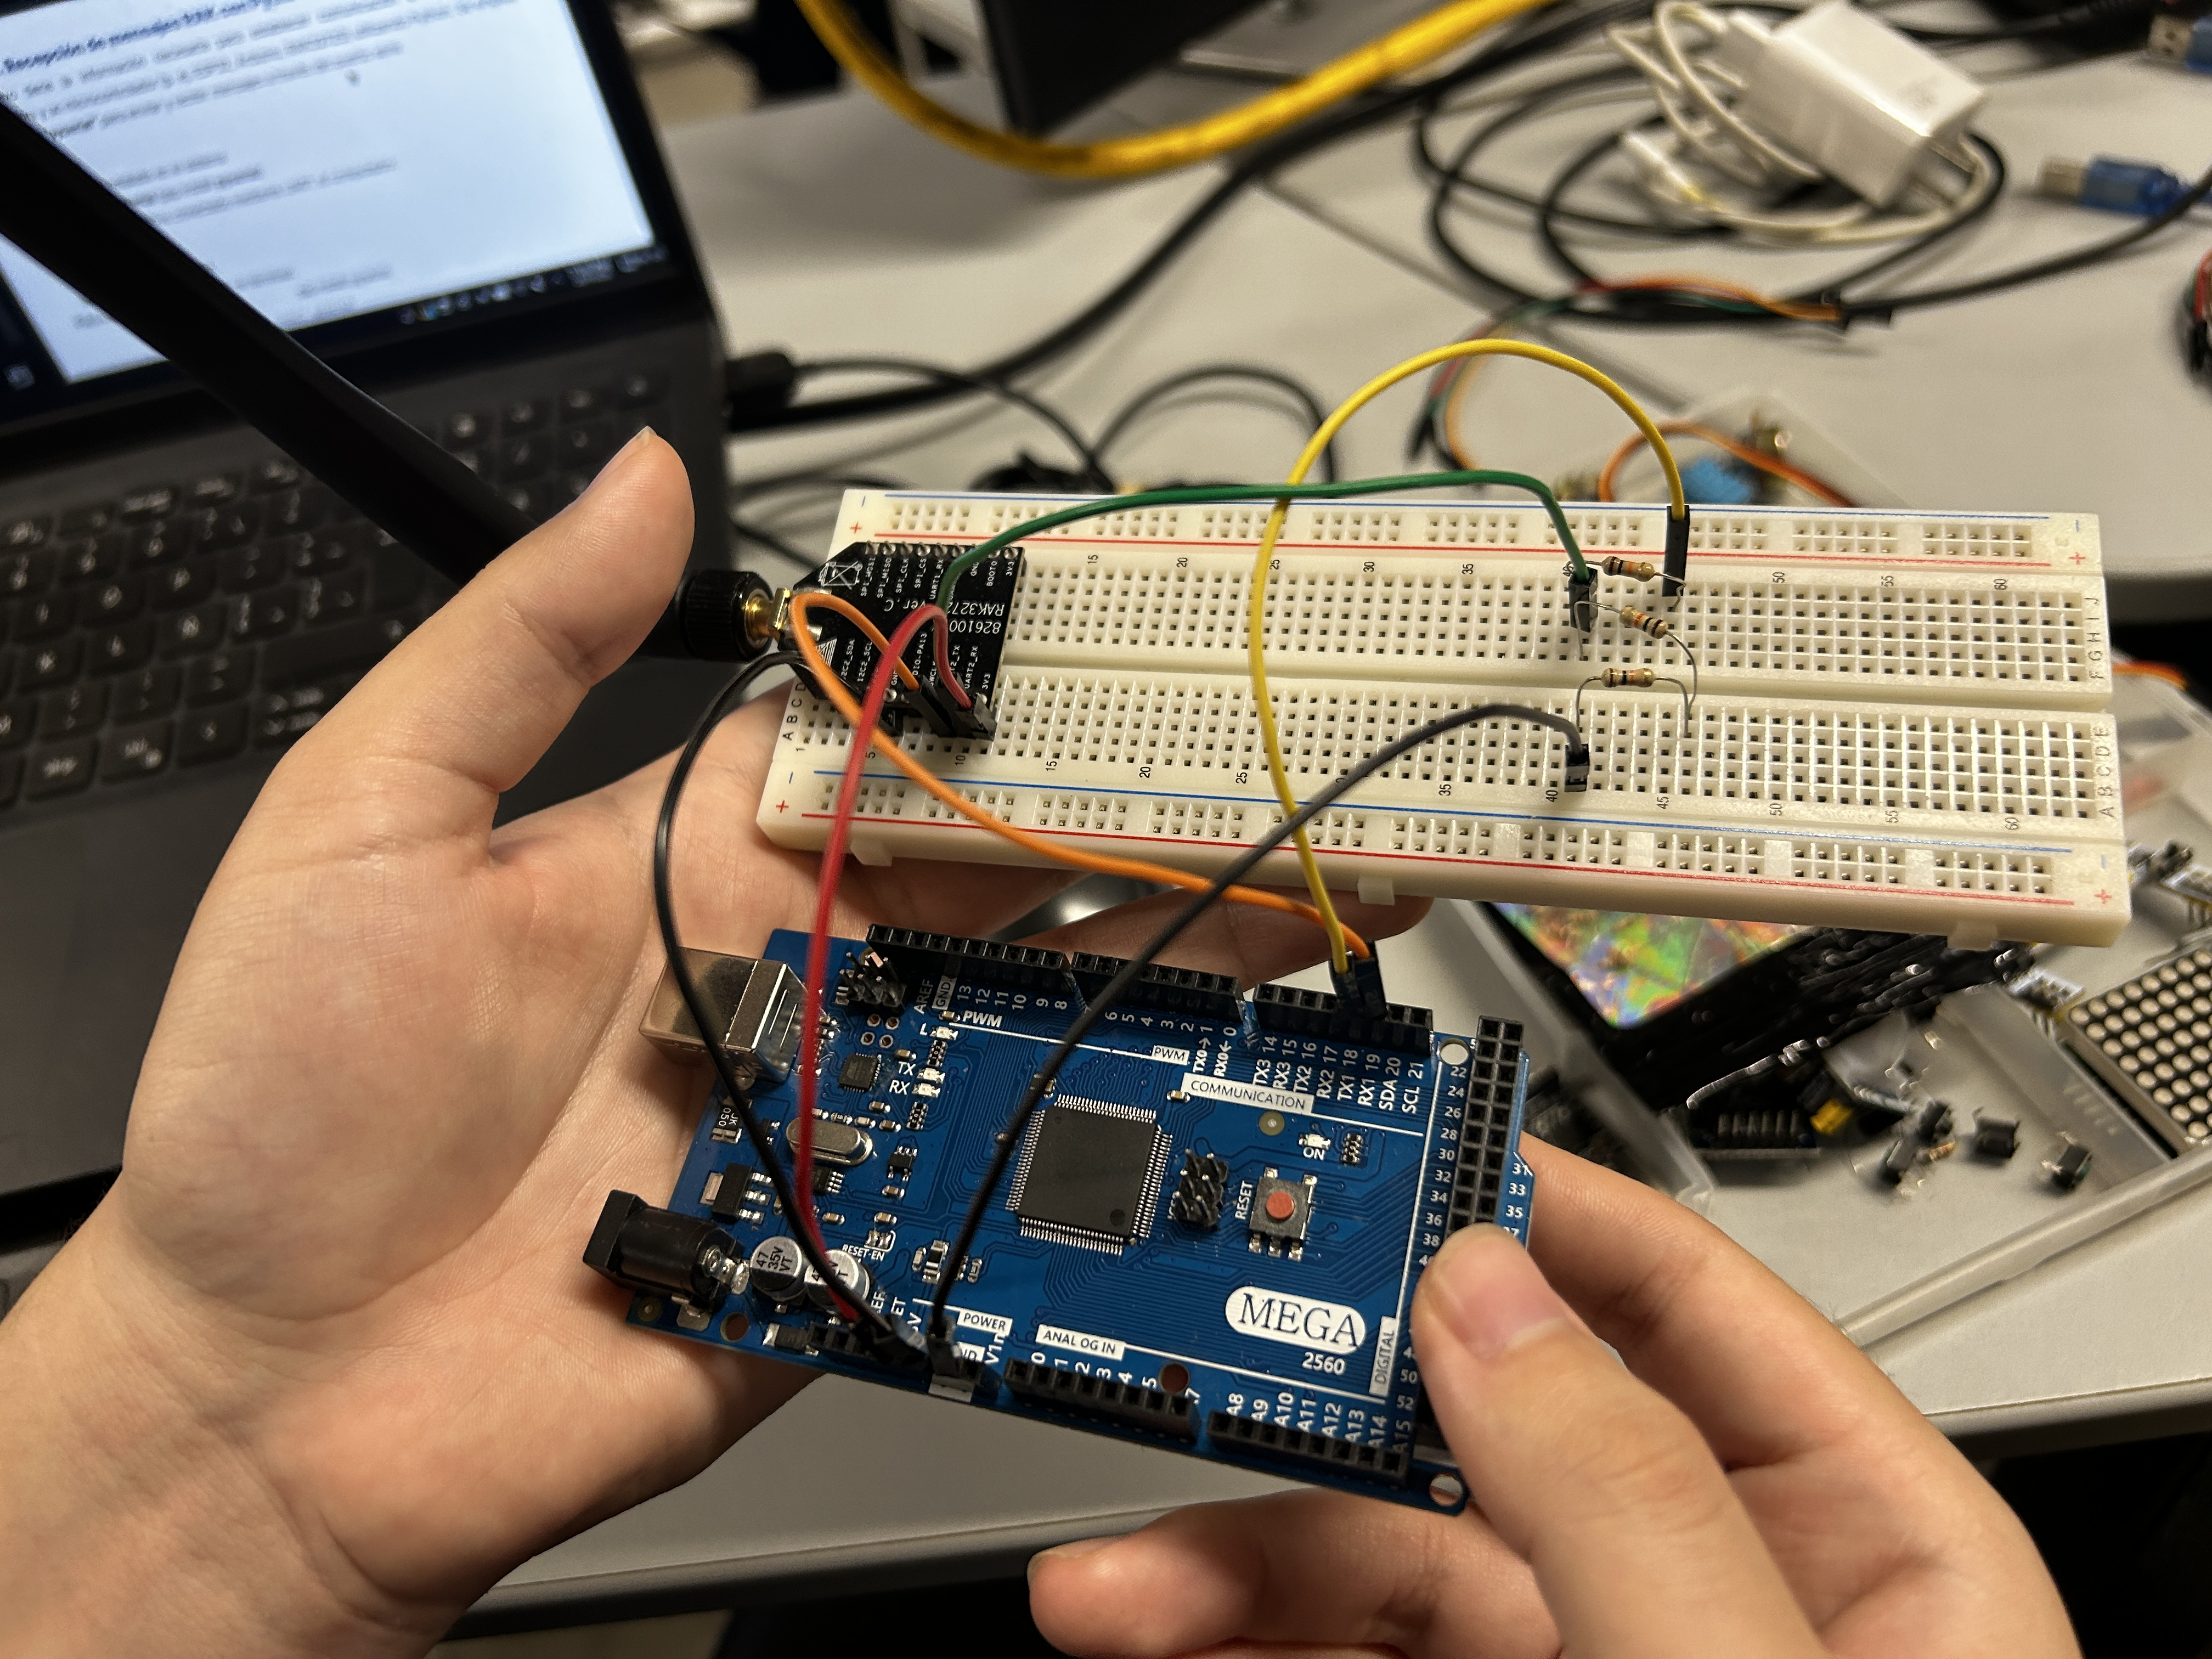
\includegraphics[width=\linewidth]{img/IMG_2478.jpg}
    \caption{Physical implementation of the Arduino MEGA and RAK LoRa module connected through a breadboard.}
    \label{fig:chk3-1}
\end{figure}

\begin{figure}[htbp]
    \centering
    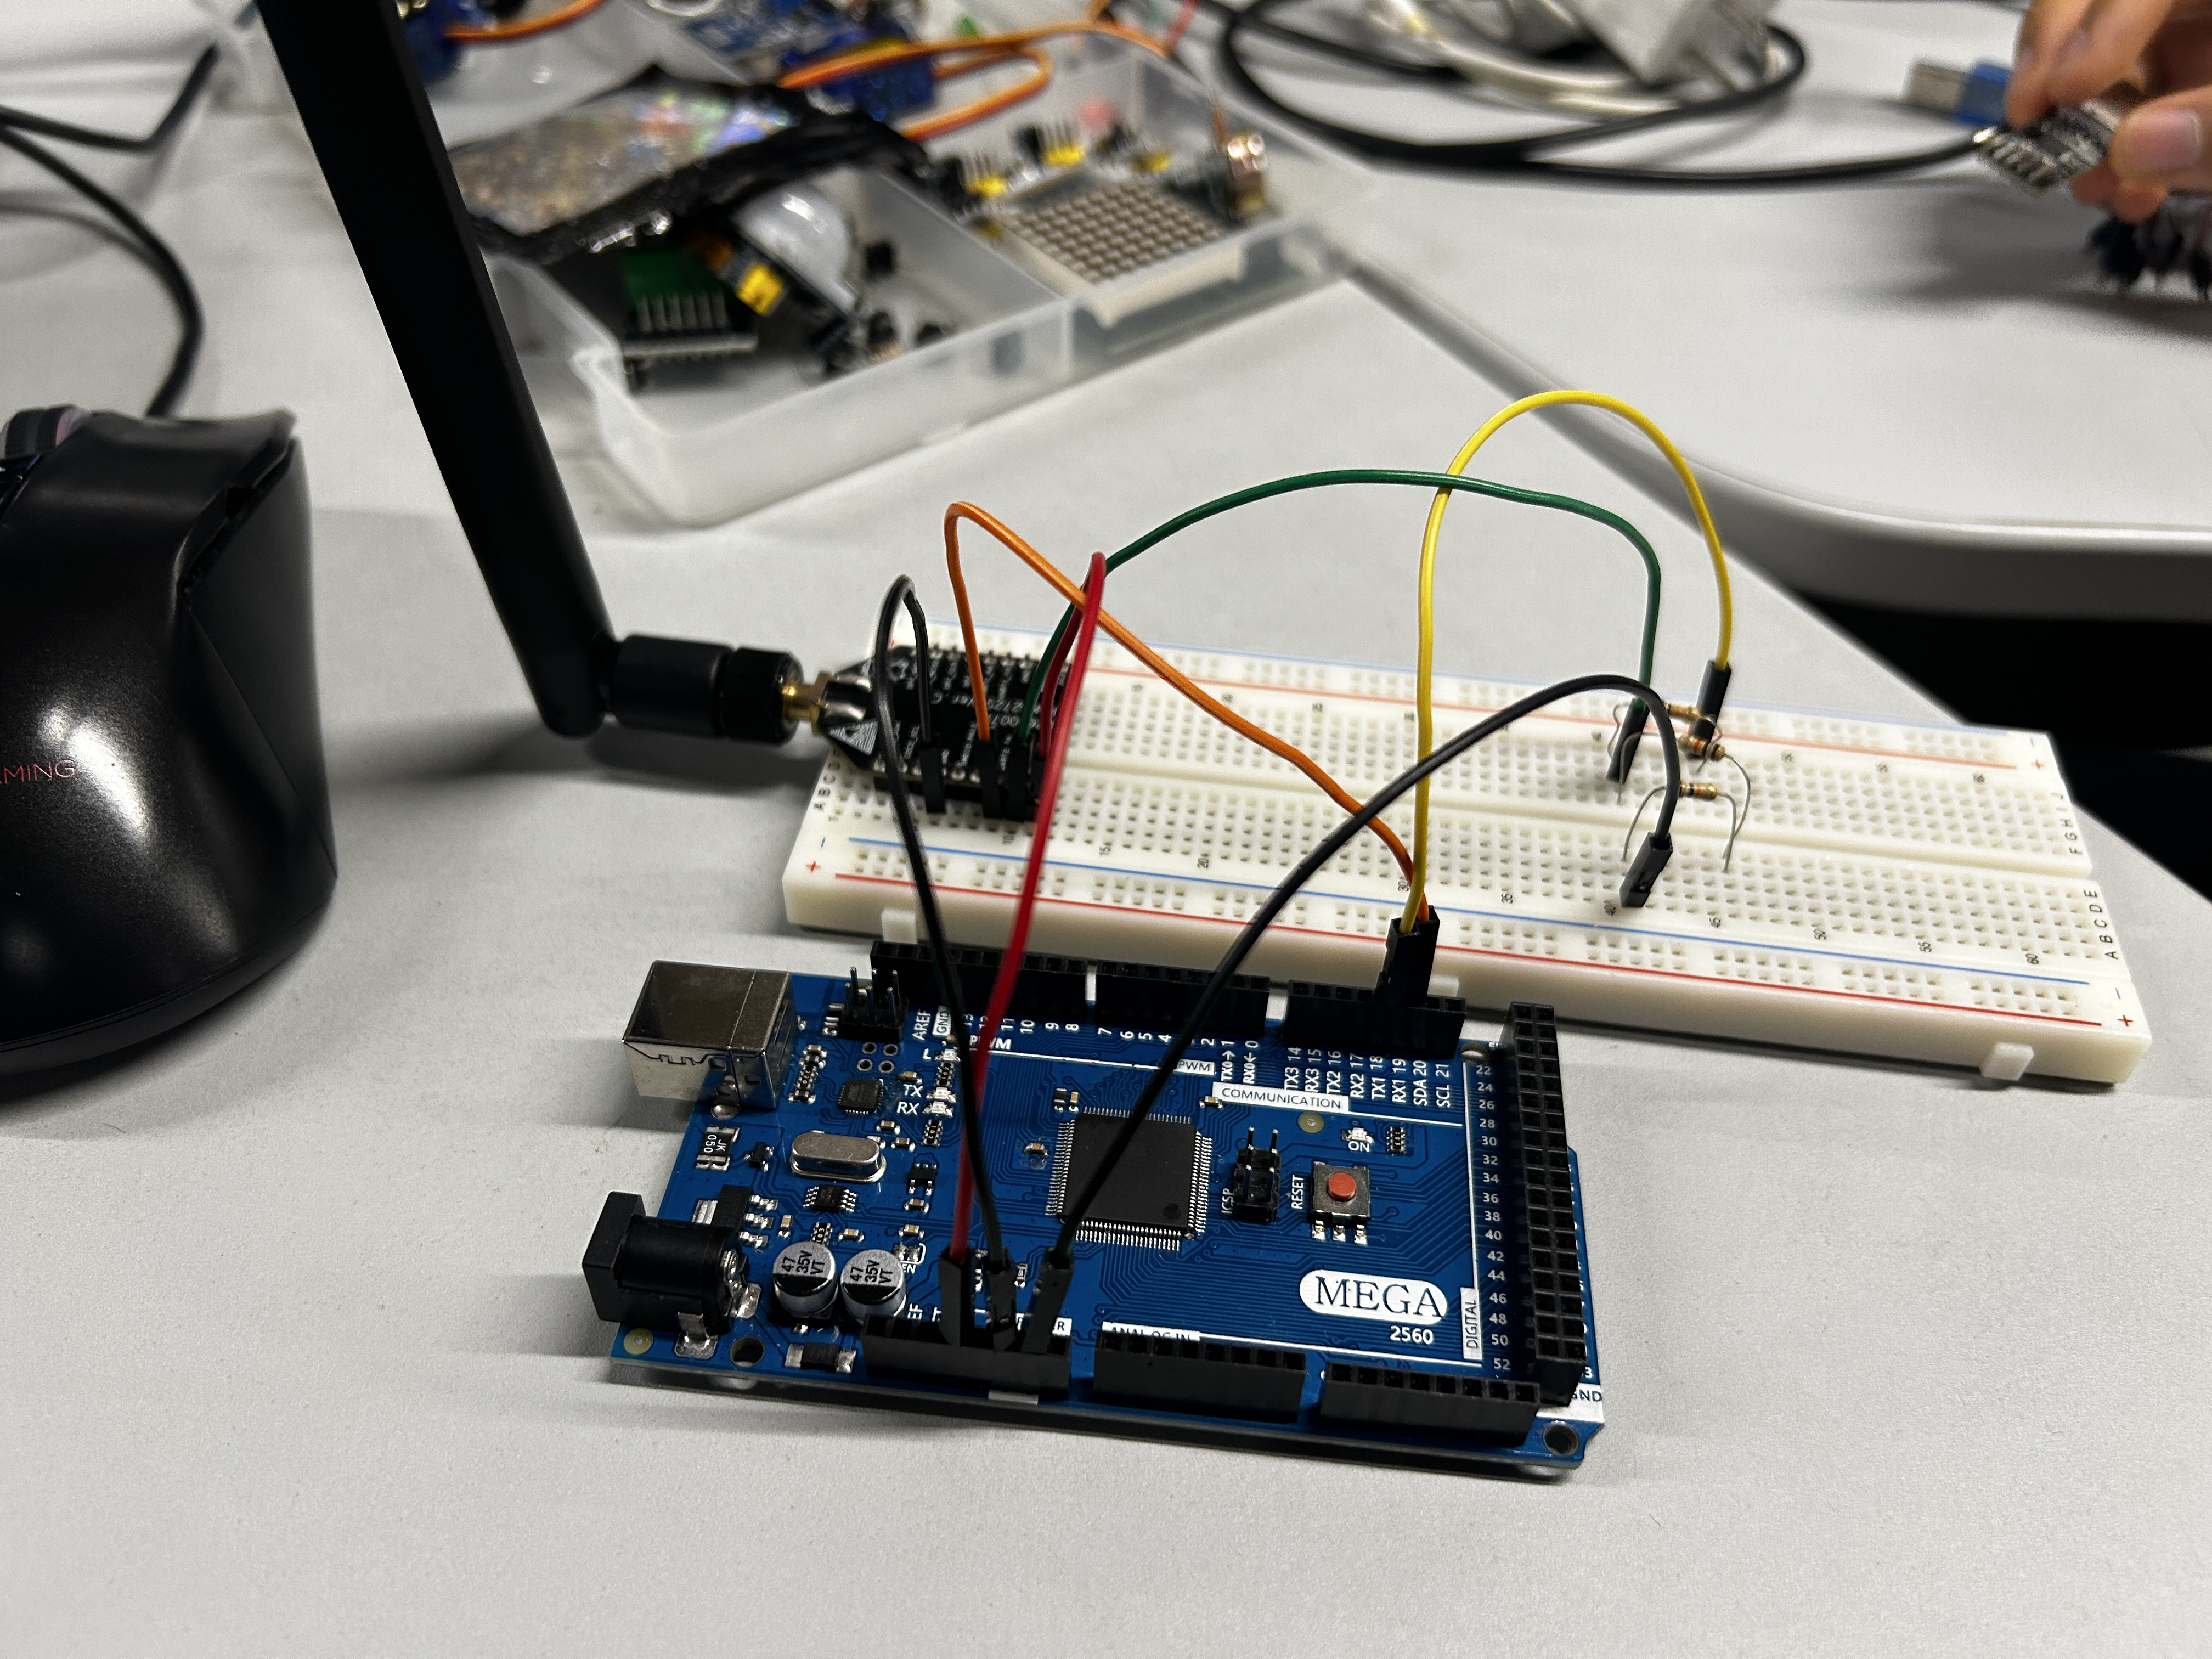
\includegraphics[width=\linewidth]{img/IMG_2479.jpg}
    \caption{Additional view of the Arduino MEGA and RAK module wiring, including the voltage divider used for UART communication.}
    \label{fig:chk3-2}
\end{figure}

\subsubsection{Arduino Code and Message Transmission}
After assembling the circuit, we developed an Arduino program to configure the RAK module and send messages automatically.
The program initializes both \texttt{Serial} and \texttt{Serial1} at 115200 baud.

The first interface is used to display information on the computer, while the second sends AT commands directly to the RAK module.
During initialization, the Arduino sends \texttt{AT+VER=?} to request the firmware version and \texttt{AT+NWM=0} to activate LoRa P2P mode.
It then configures the communication parameters using the following command:

\begin{lstlisting}[basicstyle=\ttfamily\scriptsize,breaklines=true,columns=fullflexible]
AT+P2P=923700000:12:125:0:10:14
\end{lstlisting}

This configuration establishes a frequency of 923.7 MHz, a spreading factor of 12, a bandwidth of 125 kHz, a coding rate of 4/5, a preamble length of 10, and a transmission power of 14 dBm.
Finally, \texttt{AT+PRECV=0} prepares the module for transmission.

In the main loop, the Arduino increments a counter starting from 20, converts the resulting number into its hexadecimal representation, and sends it using \texttt{AT+PSEND}.
The first transmitted counter value is 21. A delay of 5000 ms follows the response-reading function; it is a programmed pause, rather than a measured transmission period.
The program also displays the commands sent and the responses received from the RAK module, allowing us to monitor its execution through the Arduino Serial Monitor.

The shared Arduino sketch is available as \href{https://drive.google.com/file/d/1SrnPct0enrU3doz0R0MApW0z8LCoYyoH/view}{\texttt{lora.txt} in Drive} and as \texttt{code/cp3\_lora/cp3\_lora.ino}. Listing~\ref{lst:lora_sender} reproduces that source, which follows the counter example in Appendix H of the laboratory guide \cite{guide}. The payload represents generated counter data, rather than sensor measurements.

\lstinputlisting[style=arduino,caption={Shared Arduino MEGA counter program for LoRa P2P transmission.},label={lst:lora_sender}]{\labpath code/cp3_lora/cp3_lora.ino}

The shared sketch configures spreading factor 12. The sender demonstration shows \texttt{AT+P2P=923700000:10:125:0:10:14}, using spreading factor 10. These are two source-code settings, rather than parameter readbacks from both radios; neither can be assigned to the entire 108-sample receiver record.

The \texttt{sendRAK} function waits for at least one UART byte and prints the bytes available at that moment. It has no timeout and does not parse \texttt{OK} or wait specifically for \texttt{TXP2P DONE}. Completion and reception therefore need to be evaluated from the recorded radio output.


Figure~\ref{fig:chk3-sender} shows the Arduino Serial Monitor sending consecutive hexadecimal payloads, including \texttt{3332}, \texttt{3333}, and \texttt{3334}, corresponding to the text values 32, 33, and 34.
The \texttt{OK} responses and \texttt{+EVT:TXP2P DONE} events show that these transmission operations completed on the sender side.
In the sender video, the initial messages are displayed while the receiver begins moving away to test the communication range.

\begin{figure}[htbp]
    \centering
    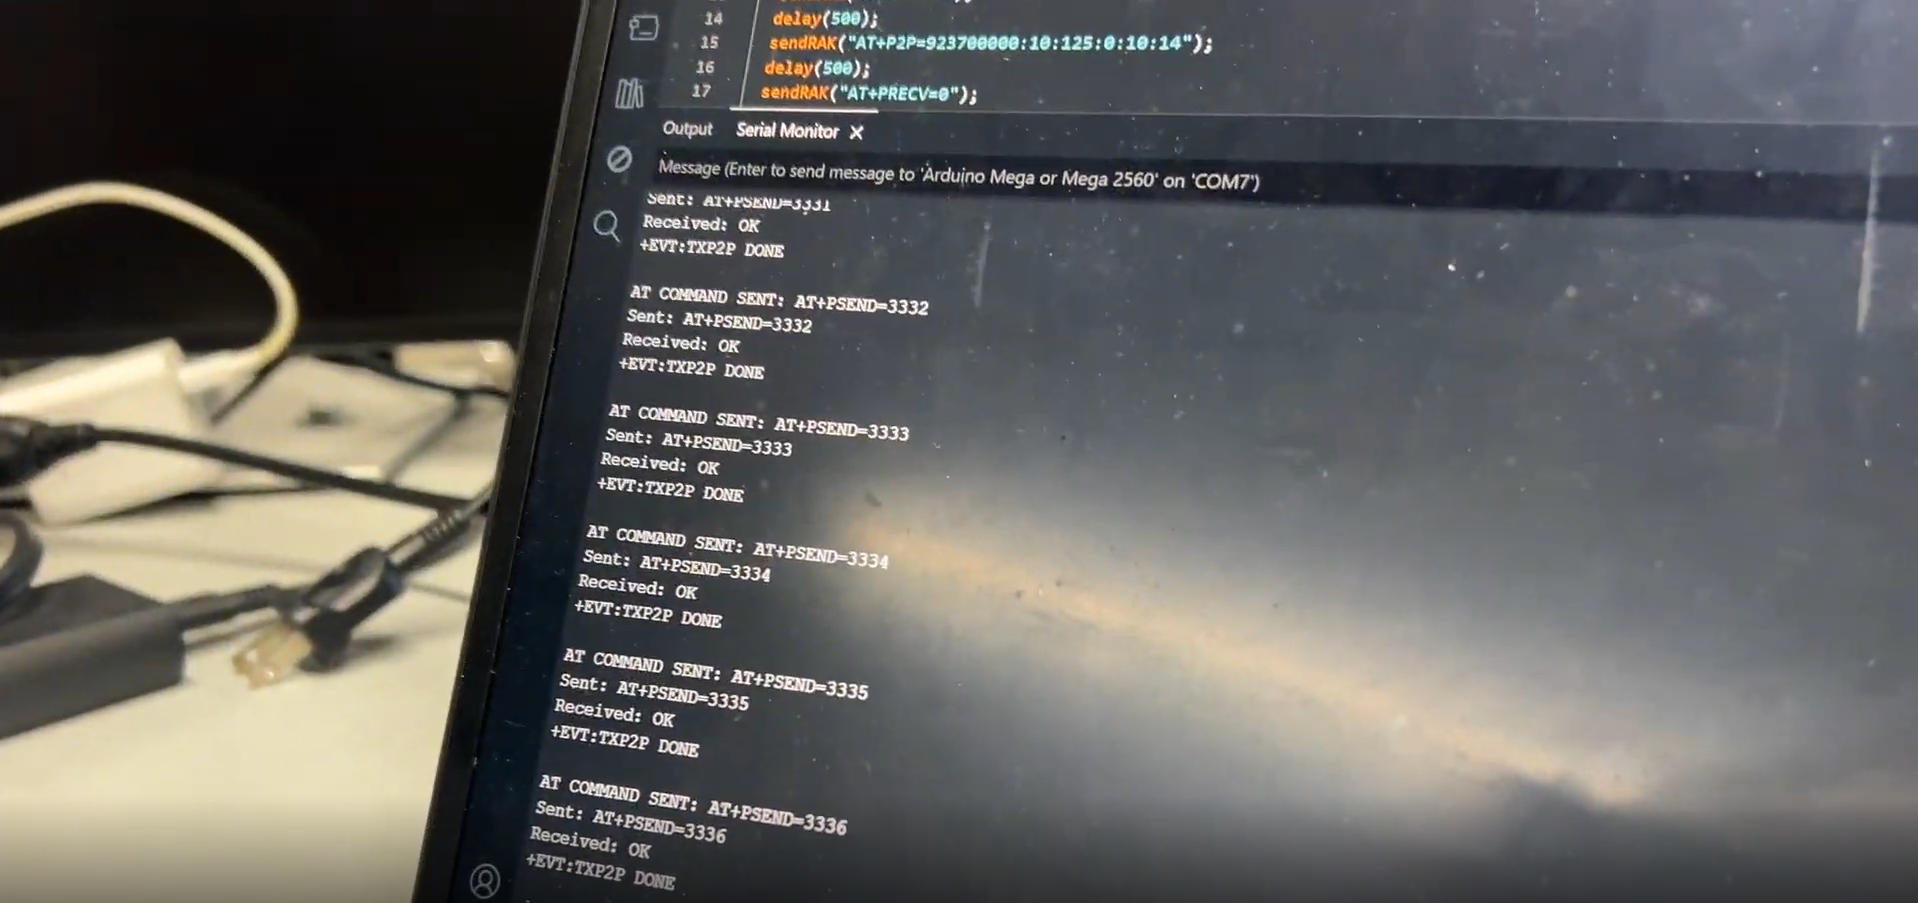
\includegraphics[width=\linewidth]{img/c3-2.png}
    \caption{Arduino MEGA Serial Monitor showing consecutive LoRa transmission commands and transmission completion events.}
    \label{fig:chk3-sender}
\end{figure}

The sender demonstration video shows the Arduino MEGA periodically issuing LoRa transmission commands while
the receiver begins moving away to test the communication range.
The Serial Monitor displays the hexadecimal payloads, the corresponding \texttt{OK} responses, and the \texttt{+EVT:TXP2P DONE} events,
confirming that the sender continued completing transmission operations during the experiment.

\noindent\textbf{Sender demonstration:}
\href{https://drive.google.com/file/d/1U7MX6kO2TPNVxZwb8u_24bP_hj0Zetdr/view}{Video sender demonstration}

Figure~\ref{fig:mega-payloads} documents another portion of the counter test, showing values 144 through 148. For example, \texttt{313434} is the hexadecimal encoding of the three ASCII characters in \texttt{144}.

\begin{figure}[htbp]
\centering
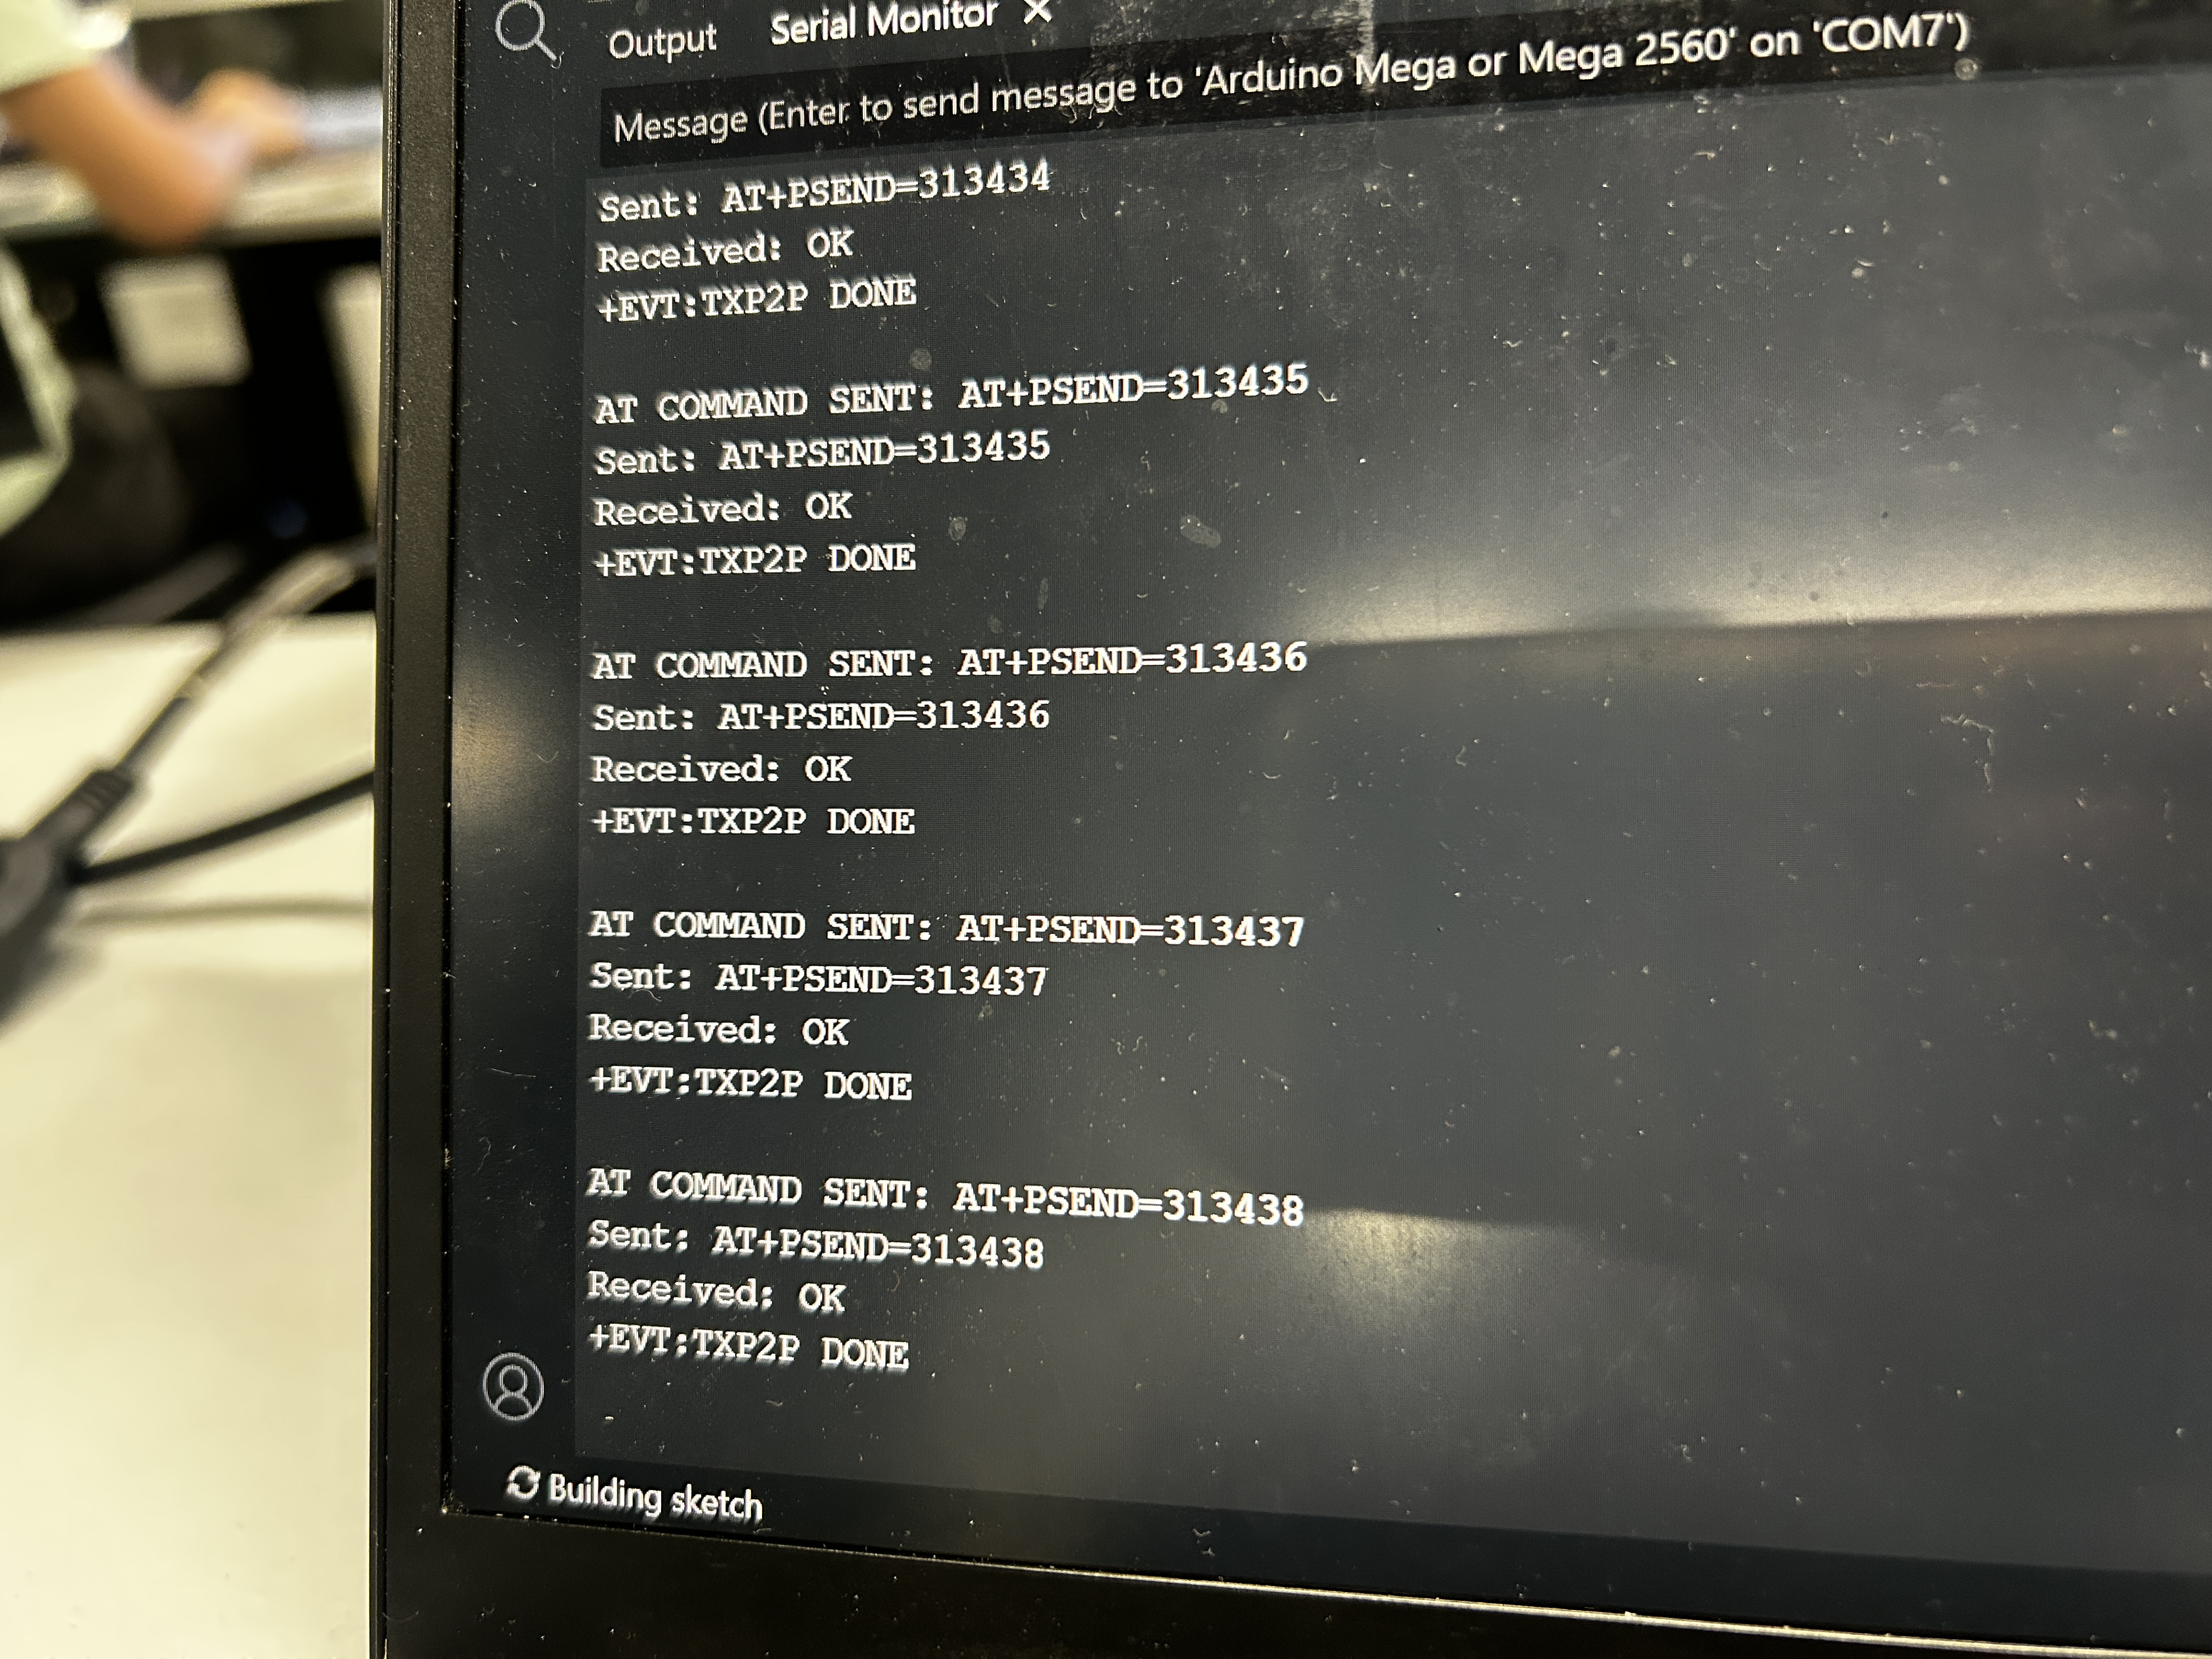
\includegraphics[width=\linewidth]{img/chk3/mega-payload-transmissions.jpg}
\caption{Serial output showing generated counter values 144--148 and local transmission-completion events.}
\label{fig:mega-payloads}
\end{figure}

\subsubsection{Reception and Discussion}

To test the automated communication, a second RAK module was connected to another computer and configured as the receiver.
Both modules used matching LoRa P2P parameters, while the receiver remained in continuous reception mode using \texttt{AT+PRECV=65534}.
The receiver was used to monitor the incoming messages and verify the communication between both devices. As shown in Figure~\ref{fig:chk3-receiver}, it displayed successive received packets and their decoded counter values, together with the corresponding RSSI and SNR measurements. For example, the visible messages include consecutive values from 21 onward, showing that the counter transmitted by the Arduino could be recovered at the receiving end. The recorded RSSI and SNR values varied between messages, illustrating changes in the received signal conditions during the test.

\begin{figure}[htbp]
    \centering
    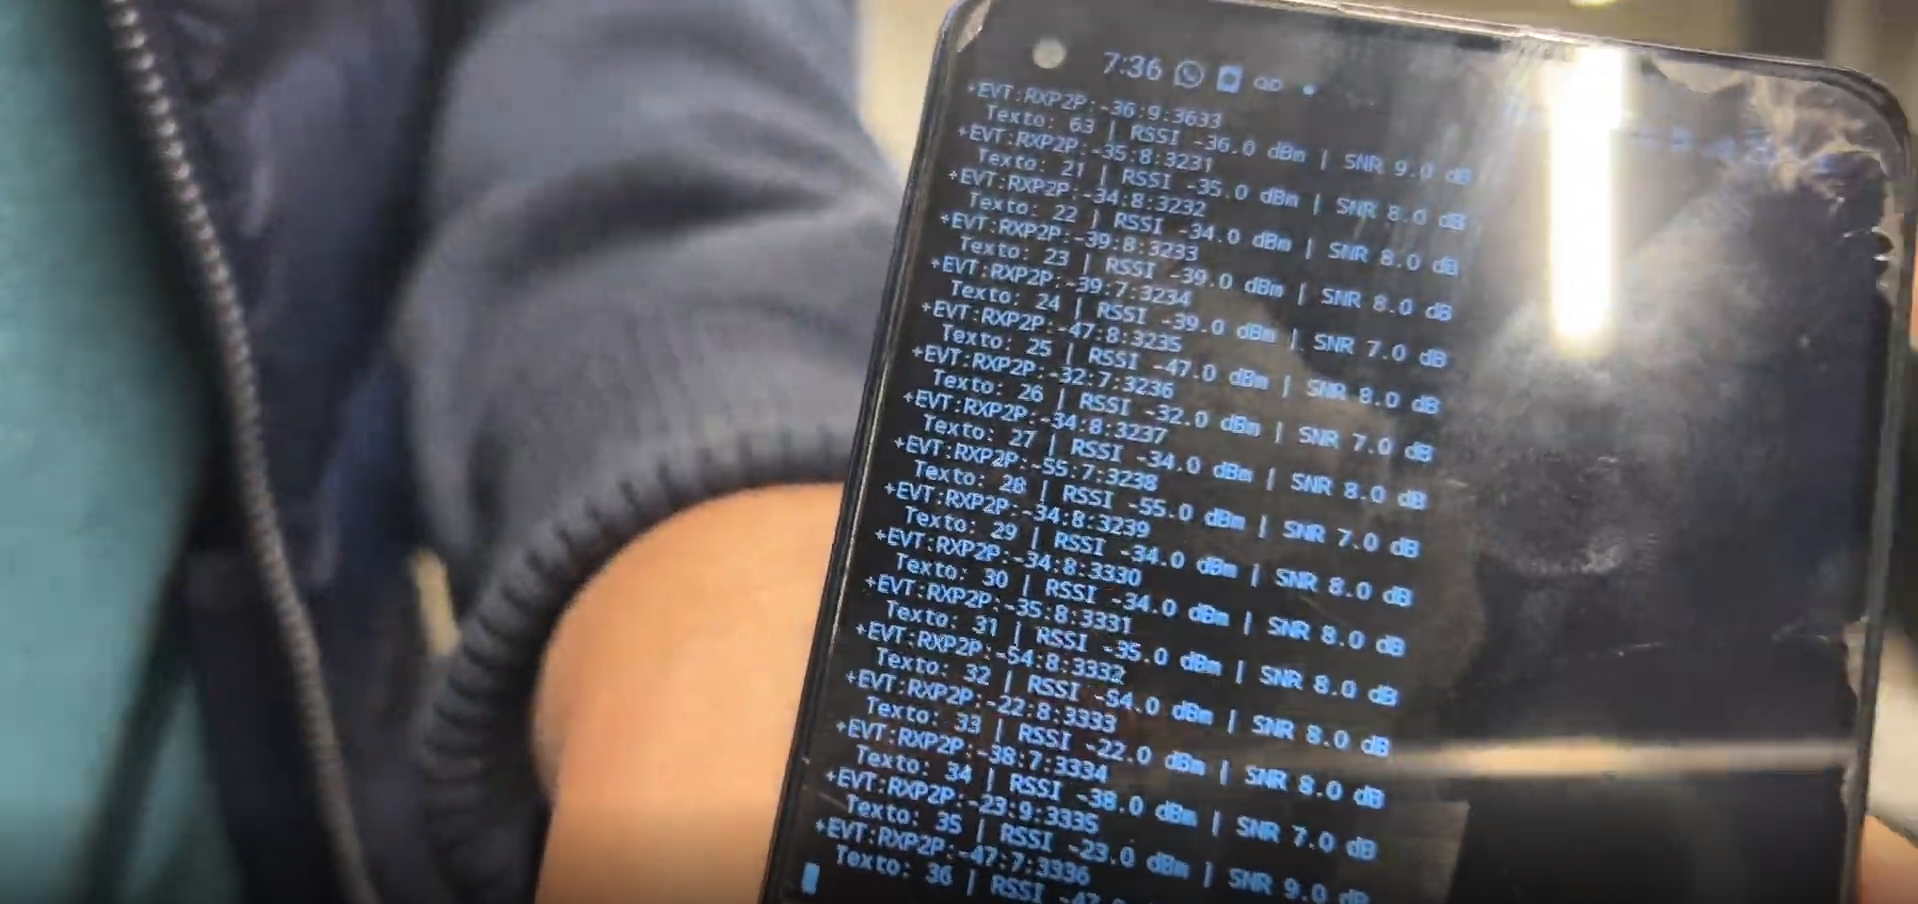
\includegraphics[width=\linewidth]{img/c3-3.png}
    \caption{Receiver terminal displaying successive decoded counter values with RSSI and SNR measurements during the LoRa range test.}
    \label{fig:chk3-receiver}
\end{figure}

As the receiver was moved farther away, the demonstration eventually showed reception errors, as illustrated in Figure~\ref{fig:chk3-loss}.
The receiver was then checked using an AT command to confirm that its serial interface was still responding.
Since messages had previously been received and the error occurred during the range test, the loss of the wireless link is consistent with the increasing separation between devices.
However, this check alone cannot completely rule out interference or other radio conditions as contributing factors.

\begin{figure}[htbp]
    \centering
    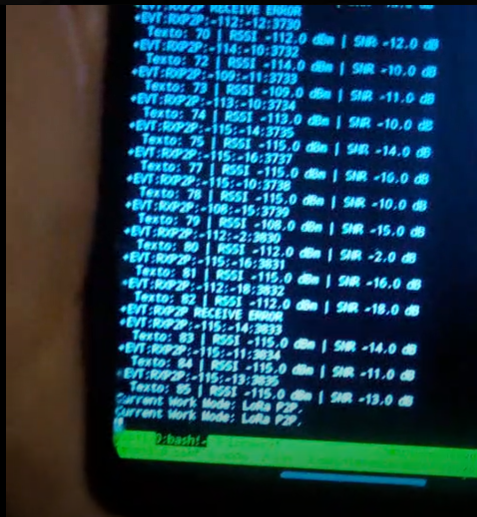
\includegraphics[width=\linewidth]{img/c3-1.png}
    \caption{Receiver terminal showing reception errors after the devices were separated during the range test, followed by a check of the module's operating mode.}
    \label{fig:chk3-loss}
\end{figure}

The receiving process is documented in two demonstration videos.
In the first video, the receiver displays consecutive messages containing the transmitted counter values, together
with their corresponding RSSI and SNR measurements.
As the receiver moves away from the sender, the incoming messages continue to be monitored, allowing us to observe
how the signal conditions change during the experiment.

\noindent\textbf{Receiver demonstration 1:}
\href{https://drive.google.com/file/d/1LbWK22VkQ3w6i1_o0mo8eUaG4k4VIdii/view}{Video receiver demonstration 1}

The second video shows a later stage of the range test, when the receiver begins displaying reception errors.
An AT command is then executed to verify that the module remains responsive.
This check is relevant because it helps distinguish a loss of wireless reception from a complete failure of the module or its serial communication.

\noindent\textbf{Receiver demonstration 2:}
\href{https://drive.google.com/file/d/1O1AkUlDwLp3YNUK6QXnnBu6x8ed5gSY3/view}{Video receiver demonstration 2}

Together, the videos and Figures~\ref{fig:chk3-receiver} and~\ref{fig:chk3-loss} provide evidence of successful
periodic reception and the communication difficulties observed as the separation between the devices increased.
Although the experiment did not establish an exact maximum distance, it demonstrated that completing a transmission
on the sender does not necessarily guarantee reception under all radio conditions.

The main achievement of this checkpoint was integrating the Arduino MEGA with the RAK module to automate LoRa communication.
While the previous checkpoint required sending each message manually, the Arduino now handles the configuration, hexadecimal conversion, and periodic transmission through its program.

An important aspect of this implementation is that the Arduino does not transmit the numerical value directly as a binary integer.
Instead, it converts the number into a text representation and then encodes each character as a hexadecimal byte.
This allows the receiving module to obtain the transmitted data in the format expected by the LoRa AT interface.

Additionally, the voltage divider was an essential part of the integration, since successful communication also depends on the electrical compatibility between the devices, not only on using the same serial protocol.

Overall, this checkpoint demonstrated both automated LoRa P2P communication and a practical limitation of the wireless link.
The Arduino continued issuing transmission commands, but reliable reception depended on the radio conditions and separation between the modules.
This distinction is important for IoT applications, where a functioning transmitter alone does not guarantee that data reaches its destination.
